\documentclass[aspectratio=169, table]{beamer}

\usepackage{colortbl}
\usepackage{xcolor}
\usepackage{listings}
\usepackage{xcolor}
\usepackage{pgfplots}
\usepgfplotslibrary{polar}
\usepackage{tikz}
\usetikzlibrary{shapes.geometric,
	positioning, shapes, shapes.multipart, backgrounds, arrows.meta, calc, fit, trees}

\usetheme{Pradita}

\lstdefinelanguage{bash} {
	keywords={},
	basicstyle=\ttfamily\scriptsize,
	keywordstyle=\color{blue}\bfseries,
	ndkeywords={iex},
	ndkeywordstyle=\color{purple}\bfseries,
	sensitive=true,
	commentstyle=\color{gray},
	stringstyle=\color{red},
	numbers=left,
	numberstyle=\tiny\color{gray},
	breaklines=true,
	frame=lines,
	backgroundcolor=\color{lightgray!10},
	tabsize=2,
	comment=[l]{\#},
	morecomment=[s]{/*}{*/},
	commentstyle=\color{gray}\ttfamily,
	stringstyle=\color{purple}\ttfamily,
	showstringspaces=false,
	captionpos=b
}

\lstdefinestyle{PythonStyle}{
    language=Python,
    basicstyle=\ttfamily\footnotesize,
    keywordstyle=\color{blue}\bfseries,
    commentstyle=\color{gray}\itshape,
    stringstyle=\color{red},
    showstringspaces=false,
    breaklines=true,
    frame=lines,
    numbers=left,
    numberstyle=\tiny\color{gray},
    backgroundcolor=\color{lightgray!10},
    tabsize=4,
    captionpos=b
}

\lstdefinelanguage{terraform} {
	keywords={variable, bool, type, number, string, default, locals, resource, dynamic,
				module, content, output},
	basicstyle=\ttfamily\scriptsize,
	keywordstyle=\color{blue}\bfseries,
	ndkeywords={iex},
	ndkeywordstyle=\color{purple}\bfseries,
	sensitive=true,
	commentstyle=\color{gray},
	stringstyle=\color{red},
	numbers=left,
	numberstyle=\tiny\color{gray},
	breaklines=true,
	frame=lines,
	backgroundcolor=\color{lightgray!10},
	tabsize=2,
	comment=[l]{\#},
	morecomment=[s]{/*}{*/},
	string=[s]{'}{'},
	morestring=[s]{"}{"},
	commentstyle=\color{gray}\ttfamily,
	stringstyle=\color{purple}\ttfamily,
	showstringspaces=false
}

\subtitle{IT30213 - Advanced Software Engineering \& DevOps}
\title{\Huge Model-based\\\vspace{8pt}
	Software Infrastructure\vspace{5pt}}
\author{\textbf{Alfa Yohannis}}

\begin{document}

\frame{\titlepage}

\begin{frame}[fragile]
	\frametitle{Contents}
	\vspace{20pt}
	\begin{columns}[t]
		\column{0.5\textwidth}
		\tableofcontents[sections={1-5}]

		\column{0.5\textwidth} 
		\tableofcontents[sections={6-20}]
	\end{columns}
\end{frame}

\begin{frame}{\hfill}
	\centering
	\Huge{\textbf{How to reduce configuration complexity 
  in software infrastructure management
  ?}}
\end{frame}

\section{Tujuan Pembelajaran}
\begin{frame}{\hfill}
	\centering
	\Huge{\textbf{Tujuan Pembelajaran}}
\end{frame}

\begin{frame}{Tujuan Pembelajaran}
\vspace{10pt}
Setelah sesi ini, mahasiswa diharapkan mampu:
\begin{enumerate}
  \item Memahami konsep \textit{Model-Driven Engineering} (MDE) untuk otomasi infrastruktur.
  \item Menjelaskan peran model, aturan transformasi, dan template dalam generasi artefak IaC.
  \item Menganalisis penerapan MDE pada proyek: dari model input hingga output Terraform dan Kubernetes.
\end{enumerate}
\end{frame}

\section{Pendahuluan dan Motivasi}
\begin{frame}{\hfill}
	\centering
	\Huge{\textbf{Pendahuluan dan Motivasi}}
\end{frame}

\begin{frame}{Mengapa Perlu Pendekatan Berbasis Model?}
\vspace{8pt}
Pada praktik DevOps modern, environment \texttt{dev}, \texttt{staging}, dan \texttt{prod}
memiliki variasi konfigurasi yang terus berkembang.

\vspace{8pt}
\textbf{Masalah umum jika edit IaC manual di banyak berkas:}
\begin{itemize}
  \item Duplikasi konfigurasi.
  \item Deviasi antar environment (\textit{config drift}).
  \item Perubahan global sulit dan rawan error.
  \item Jejak keputusan teknis kurang jelas.
\end{itemize}

\vspace{6pt}
MDE menaikkan level abstraksi: konfigurasi dipusatkan di model,
lalu artefak teknis dihasilkan otomatis.
\end{frame}

\section{Konsep Dasar MDE}
\begin{frame}{\hfill}
	\centering
	\Huge{\textbf{Konsep Dasar MDE}}
\end{frame}

\begin{frame}{Metamodel, Model, dan Instance}
\vspace{8pt}
\centering
\scalebox{0.65}{%
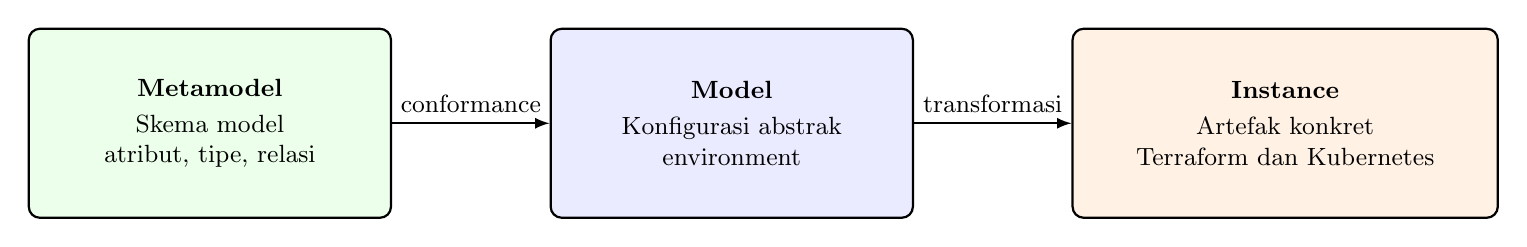
\begin{tikzpicture}[
  font=\small,
  >=latex,
  thick,
  box/.style={draw, rounded corners, minimum width=4.6cm, minimum height=2.4cm, align=center},
  lbl/.style={align=center}
]
  \node[box, fill=green!8] (metamodel) {
    \textbf{Metamodel}\\[2pt]
    Skema model\\atribut, tipe, relasi
  };

  \node[box, fill=blue!8, right=20mm of metamodel] (model) {
    \textbf{Model}\\[2pt]
    Konfigurasi abstrak\\environment
  };

  \node[box, fill=orange!10, right=20mm of model, minimum width=5.4cm] (instance) {
    \textbf{Instance}\\[2pt]
    Artefak konkret\\Terraform dan Kubernetes
  };

  \draw[->] (metamodel.east) -- (model.west) node[midway, above, lbl] {conformance};
  \draw[->] (model.east) -- (instance.west) node[midway, above, lbl] {transformasi};
\end{tikzpicture}
}%

\vspace{8pt}
\small
Satu model valid dapat diturunkan menjadi banyak instance deployment
secara konsisten.
\end{frame}

\begin{frame}{Pemodelan Tekstual dan Generasi Kode}
\vspace{8pt}
\textbf{Pemodelan tekstual (YAML):}
\begin{itemize}
  \item Mudah dibaca manusia, mudah diproses mesin.
  \item Natural untuk \textit{version control} dan \textit{code review}.
  \item Mudah diintegrasikan ke pipeline CI/CD.
\end{itemize}

\vspace{6pt}
\textbf{Alur kerja generasi artefak:}
\begin{enumerate}
  \item Update model environment.
  \item Jalankan generator berbasis template.
  \item Verifikasi artefak hasil generasi.
  \item Provision/deploy ke environment target.
\end{enumerate}
\end{frame}

\section{Keuntungan dan Kerugian MDE}
\begin{frame}{\hfill}
	\centering
	\Huge{\textbf{Keuntungan dan Kerugian MDE}}
\end{frame}

\begin{frame}{Trade-off Pendekatan MDE}
\vspace{8pt}
\begin{columns}[T]
\column{0.5\textwidth}
\textbf{Keuntungan}
\begin{itemize}
  \item Konsistensi artefak lintas environment.
  \item Mengurangi duplikasi konfigurasi.
  \item Ketertelusuran perubahan lebih baik.
  \item Penambahan varian baru lebih cepat.
  \item Standardisasi praktik tim meningkat.
\end{itemize}

\column{0.5\textwidth}
\textbf{Kerugian}
\begin{itemize}
  \item Biaya adopsi awal relatif tinggi.
  \item Debugging multi-lapisan lebih kompleks.
  \item Butuh disiplin desain model dan template.
  \item Risiko \textit{over-engineering} untuk domain sederhana.
\end{itemize}
\end{columns}
\end{frame}

\section{MDE di Industri dan DevOps}
\begin{frame}{\hfill}
	\centering
	\Huge{\textbf{MDE di Industri dan DevOps}}
\end{frame}

\begin{frame}{Contoh Aplikasi MDE di Dunia Industri}
\vspace{8pt}
\textbf{Sektor penggunaan umum:}
\begin{itemize}
  \item Otomotif: arsitektur ECU, AUTOSAR, variasi produk kendaraan.
  \item Aviasi/pertahanan: \textit{model-based systems engineering}, traceability requirement.
  \item Manufaktur/otomasi: \textit{digital twin}, konfigurasi sistem kontrol.
\end{itemize}

\vspace{8pt}
\textbf{Contoh perusahaan:}
Siemens, Bosch, BMW Group, Mercedes-Benz, Volkswagen Group, Airbus,
Boeing, ABB, Schneider Electric.
\end{frame}

\begin{frame}{Potensi MDE dalam Praktik DevOps}
\vspace{8pt}
\textbf{Integrasi CI/CD:}
\begin{itemize}
  \item Validasi model/metamodel di tahap awal.
  \item Transformasi model ke artefak IaC di tahap build.
  \item Verifikasi sintaks dan kebijakan sebelum deployment.
\end{itemize}

\vspace{8pt}
\textbf{Dampak utama:}
\begin{itemize}
  \item Governance lebih kuat (aturan ditanam di metamodel/template).
  \item Compliance lebih konsisten lintas environment.
  \item Skalabilitas operasional multi-tim lebih terjaga.
\end{itemize}
\end{frame}

\section{Pendekatan MDE pada Proyek}
\begin{frame}{\hfill}
	\centering
	\Huge{\textbf{Pendekatan MDE pada Proyek}}
\end{frame}

\begin{frame}{Arsitektur Pendekatan Berbasis Model}
\vspace{4pt}
\centering
\scalebox{0.58}{%
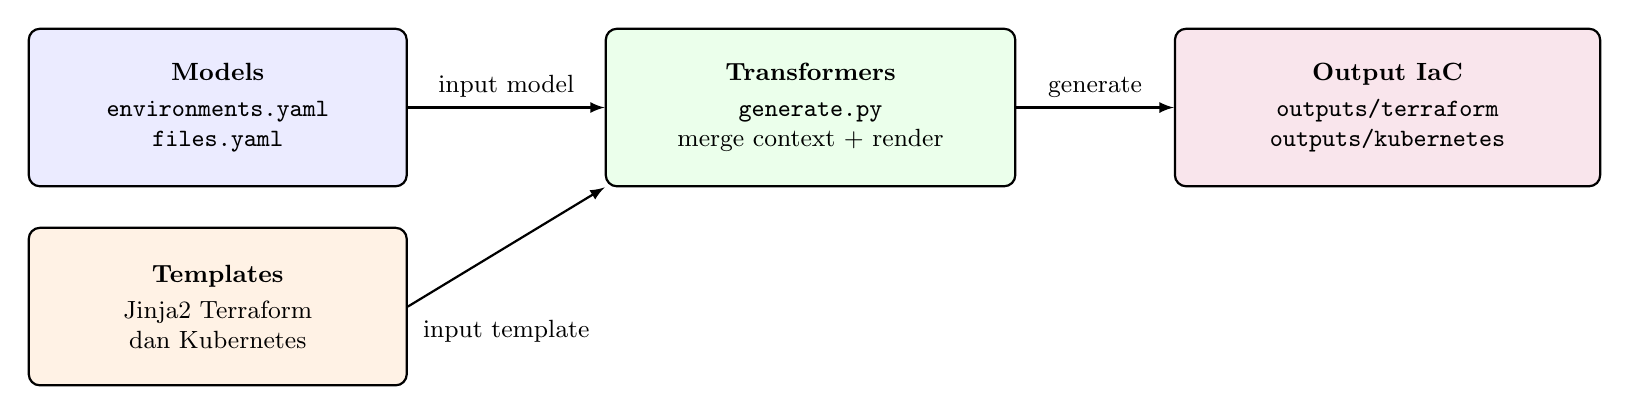
\begin{tikzpicture}[
  font=\small,
  >=latex,
  thick,
  box/.style={draw, rounded corners, minimum width=4.8cm, minimum height=2cm, align=center},
  lbl/.style={align=center}
]
  \node[box, fill=blue!8] (models) {
    \textbf{Models}\\[2pt]
    \texttt{environments.yaml}\\\texttt{files.yaml}
  };

  \node[box, fill=orange!10, below=5mm of models] (templates) {
    \textbf{Templates}\\[2pt]
    Jinja2 Terraform\\dan Kubernetes
  };

  \node[box, fill=green!8, right=25mm of models, minimum width=5.2cm] (transformers) {
    \textbf{Transformers}\\[2pt]
    \texttt{generate.py}\\merge context + render
  };

  \node[box, fill=purple!10, right=20mm of transformers, minimum width=5.4cm] (output) {
    \textbf{Output IaC}\\[2pt]
    \texttt{outputs/terraform}\\\texttt{outputs/kubernetes}
  };

  \draw[->] (models.east) -- (transformers.west) node[midway, above, lbl] {input model};
  \draw[->] (templates.east) -- (transformers.south west) node[midway, below, lbl, yshift=-8mm] {input template};
  \draw[->] (transformers.east) -- (output.west) node[midway, above, lbl] {generate};
\end{tikzpicture}
}%
\end{frame}

\begin{frame}[fragile]{Komponen Folder \texttt{mde}}
\vspace{8pt}
\begin{lstlisting}[language=bash]
mde/
|-- README.md
|-- models/
|   |-- environments.yaml
|   `-- files.yaml
|-- transformers/
|   |-- generate.py
|   `-- requirements.txt
`-- templates/
    |-- core/
    |   |-- terraform/modules/tts_stack/*.j2
    |   `-- kubernetes/base/*.j2
    |-- terraform/env/*.j2
    `-- kubernetes/overlay/*.j2
\end{lstlisting}
\end{frame}

\begin{frame}{Model dari Definisi Variasi Environment}
\vspace{20pt}
\centering
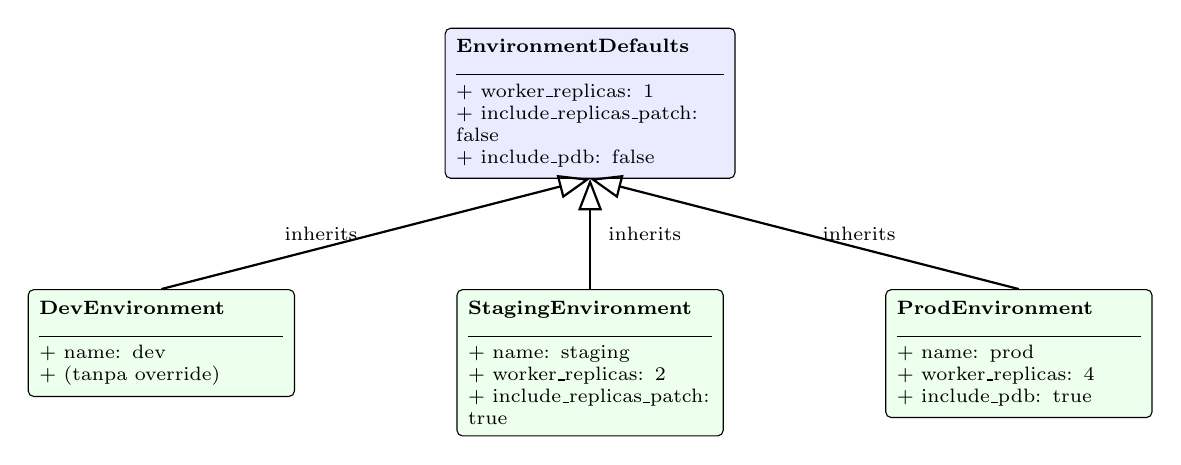
\begin{tikzpicture}[
  classbox/.style={draw, rounded corners=2pt, align=left, font=\scriptsize, inner sep=4pt},
  basebox/.style={classbox, fill=blue!8, text width=3.4cm},
  envbox/.style={classbox, fill=green!7, text width=3.1cm},
  inh/.style={-{Triangle[open, length=4mm, width=3mm]}, thick}
]
\node[basebox] (base) {
  \textbf{EnvironmentDefaults}\\
  \rule{\linewidth}{0.2pt}\\
  + worker\_replicas: 1\\
  + include\_replicas\_patch: false\\
  + include\_pdb: false
};

\node[envbox, below left=14mm and 19mm of base] (dev) {
  \textbf{DevEnvironment}\\
  \rule{\linewidth}{0.2pt}\\
  + name: dev\\
  + (tanpa override)
};

\node[envbox, below=14mm of base] (stg) {
  \textbf{StagingEnvironment}\\
  \rule{\linewidth}{0.2pt}\\
  + name: staging\\
  + worker\_replicas: 2\\
  + include\_replicas\_patch: true
};

\node[envbox, below right=14mm and 19mm of base] (prod) {
  \textbf{ProdEnvironment}\\
  \rule{\linewidth}{0.2pt}\\
  + name: prod\\
  + worker\_replicas: 4\\
  + include\_pdb: true
};

\draw[inh] (dev.north) -- (base.south) node[midway, left, xshift=-1mm] {\scriptsize inherits};
\draw[inh] (stg.north) -- (base.south) node[midway, right, xshift=1mm] {\scriptsize inherits};
\draw[inh] (prod.north) -- (base.south) node[midway, right, xshift=1mm] {\scriptsize inherits};
\end{tikzpicture}

\vspace{5pt}
\scriptsize
Setiap environment mewarisi atribut dari \texttt{defaults}; nilai yang didefinisikan ulang menjadi override spesifik environment.
\end{frame}

\begin{frame}[fragile]{Contoh Model dan Aturan Transformasi}
\vspace{6pt}
\begin{columns}[T]
\column{0.52\textwidth}
\textbf{Model (\texttt{environments.yaml})}
\begin{lstlisting}[language=bash]
defaults:
  worker_replicas: 1
  include_replicas_patch: false
  include_pdb: false

environments:
  - name: dev
  - name: staging
    worker_replicas: 2
    include_replicas_patch: true
\end{lstlisting}

\column{0.48\textwidth}
\textbf{Pola transformasi (\texttt{generate.py})}
\begin{itemize}
  \item Merge \textit{defaults} + override env.
  \item Bentuk atribut turunan.
  \item Evaluasi kondisi \texttt{when}.
  \item Render template Jinja2 ke output.
\end{itemize}
\end{columns}
\end{frame}

\section{Demo Generasi Artefak}
\begin{frame}{\hfill}
	\centering
	\Huge{\textbf{Demo Generasi Artefak}}
\end{frame}

\begin{frame}[fragile]{Langkah Eksekusi Generator}
\vspace{8pt}
\begin{lstlisting}[language=bash]
cd mde/transformers
pip install -r requirements.txt
python generate.py
\end{lstlisting}

\vspace{6pt}
\textbf{Verifikasi hasil:}
\begin{lstlisting}[language=bash]
tree ../../outputs
ls -la ../../outputs/terraform
ls -la ../../outputs/kubernetes
\end{lstlisting}
\end{frame}

\begin{frame}[fragile]{Contoh Manfaat Praktis Multi-Environment}
\vspace{8pt}
\begin{itemize}
  \item Ubah nilai \texttt{worker\_replicas} pada model \texttt{staging}.
  \item Jalankan ulang generator.
  \item Artefak patch replica hanya muncul jika kondisi \texttt{when} terpenuhi.
\end{itemize}

\vspace{6pt}
\begin{lstlisting}[language=bash]
# contoh validasi cepat
rg "replicas" outputs/kubernetes/overlays/staging
rg "PodDisruptionBudget" outputs/kubernetes/overlays/prod
\end{lstlisting}

\vspace{6pt}
\small
Inti demo: variasi environment dikelola di level model, bukan dengan copy-paste YAML.
\end{frame}

\section{Ringkasan}
\begin{frame}{\hfill}
	\centering
	\Huge{\textbf{Ringkasan}}
\end{frame}

\begin{frame}{Kesimpulan Sesi}
\vspace{8pt}
\begin{itemize}
  \item MDE menempatkan model sebagai \textit{single source of truth} konfigurasi infrastruktur.
  \item Transformasi dan template menghasilkan artefak Terraform/Kubernetes yang konsisten.
  \item Pendekatan ini relevan untuk DevOps multi-environment karena mengurangi drift dan duplikasi.
  \item Trade-off utama ada pada investasi awal desain model dan pipeline generator.
  \item Pada proyek ini, folder \texttt{mde} menunjukkan implementasi MDE yang konkret dan dapat diaudit.
\end{itemize}
\end{frame}

\end{document}
